\documentclass[sigconf,anonymous,review]{acmart}
% acmart already loads: inputenc, fontenc, hyperref, url, microtype, graphicx,
% xcolor, amsmath, amsfonts, booktabs, natbib. Do NOT re-load these or the
% \usepackage{cite} package, which conflicts with acmart's natbib.
\usepackage{multirow}
\usepackage{nicefrac}
\usepackage{tikz}
\usepackage{placeins}
\usepackage{etoolbox}
\usepackage{algorithm}
\usepackage{algpseudocode}
\usetikzlibrary{positioning, arrows.meta, shapes.geometric, calc, backgrounds, fit}
\newcommand{\TODO}[1]{\textcolor{red}{\textbf{[TODO: #1]}}}

% Strip the ACM reference / copyright footer for the anonymous review build.
\settopmatter{printacmref=false}
\setcopyright{none}
\renewcommand\footnotetextcopyrightpermission[1]{}
\pagestyle{plain}
\acmConference[Conference'26]{}{2026}{}
\acmYear{2026}
\copyrightyear{2026}

\title{FADO: A Reaction Controller for Fairness-Aware Online Learning Under Concept Drift}

\author{Anonymous}
\affiliation{%
  \institution{Anonymous}
  \country{}}
\email{anonymous@example.com}

\begin{document}


\begin{abstract}
  Online learning systems in non-stationary environments must stay both predictive and fair as the data distribution evolves, yet existing fairness-aware learners
  optimise a fixed regulariser and ignore concept drift, while drift-adaptive streaming methods enforce no fairness. We propose Fairness-Aware Drift-Aware Online
  Learning (\textsc{FADO}), which couples the \textsc{Aranyani} fair oblique decision forest~\cite{chowdhury2024enhancing} with a dual-threshold ADWIN detector and a
  reaction controller that spikes the learning rate and sharpens the soft-routing temperature on confirmed drift, annealing both back during recovery. We target the
  \emph{multi-attribute} setting, optimising the \emph{intersectional} demographic parity (DP) over the Cartesian-product subgroups of two protected attributes rather
  than each axis alone --- necessary to avoid the fairness-gerrymandering loophole of marginal-only regularisation. On \textsc{Folktables} ACS Income (CA), a natural
  $2015\!\to\!2017$--$18$ cross-year shift with sex\,$\times$\,race grouping, aggregated over $30$ seeds, \textsc{FADO} attains the best intersectional and marginal DP
  against the \textsc{ARF} and \textsc{RFR} streaming baselines and a controller-free \textsc{Aranyani} ablation, beating every baseline at paired Wilcoxon Holm-corrected
  $p<0.001$ --- including a both-tests-significant reduction over the controller-free baseline that the single-attribute setting did not surface --- at a negligible
  ($\le\!0.3$pp, Welch $p=0.10$) accuracy cost, more than halving the DP of \textsc{ARF} and \textsc{RFR}. We further find that the fair learners carry the highest
  residual intersectional-to-marginal disparity ratio, empirically confirming the gerrymandering risk intersectional optimisation removes. Direct equalised-odds
  optimisation and the intersectional \textsc{COMPAS} testbed are the subject of an ongoing companion sweep.
\end{abstract}

\keywords{fairness-aware online learning, concept drift, intersectional
fairness, oblique decision forests, drift detection}

\maketitle

\section{Introduction}
The increasing deployment of machine learning (ML) systems in high-stakes decision-making domains, including healthcare~\cite{8474918}, criminal justice~\cite{10467221}, 
and hiring~\cite{10.1145/3351095.3372828}, where their predictions may directly affect individuals and society makes optimizing for performance an insufficient objective; 
models must also satisfy fairness requirements to ensure equitable treatment across individuals or groups of individuals~\cite{10.1145/3457607}. In this regard,  
among the fairness literature, \emph{group fairness}~\cite{10.1145/2090236.2090255} has emerged as one of the most widely studied paradigms, aiming to ensure that predictive behaviour is
balanced across populations defined by sensitive attributes such as gender, race, or age. Common formulations include demographic parity, equal 
opportunity, and equalized odds, each imposing statistical constraints on model outcomes across groups (sometimes mutual incompatible)~\cite{10.1145/2090236.2090255,NIPS2016_6a9659fe}.
Most existing fairness-aware models, however, are developed under the assumption of a stationary data distribution. In practice, 
real-world environments are inherently dynamic, and the statistical properties of data may evolve over time due to policy changes, behavioural 
shifts, seasonal effects, economic fluctuations, or other social transformations. This phenomenon, commonly referred to as concept drift, 
occurs when the relationship between input variables and target outcomes changes over time, causing previously learned decision boundaries to 
become outdated. Different forms of concept drift~\cite{DBLP:journals/corr/WebbHCNP15} require different adaptation strategies and can degrade performance when models fail to adjust. 
Drift also threatens fairness: shifting distributions alter the statistical relationships that support fairness guarantees, increasing bias against some groups.
To address this challenge, the online learning and data stream mining literature has proposed numerous adaptive methods capable of detecting and 
responding to concept drift in real time. These approaches often rely on drift detection mechanisms combined with incremental learning 
strategies to maintain predictive accuracy under non-stationary conditions. Nevertheless, the majority of existing methods focus primarily on 
predictive utility~\cite{10.1007/s10994-017-5642-8, KLAIBER20231261}, while fairness considerations remain comparatively underexplored. As a result, fairness guarantees established during training 
may deteriorate over time even when predictive accuracy remains relatively stable~\cite{Deho2025}. This limitation is particularly critical in high-stakes applications, 
where persistent fairness violations may remain undetected for extended periods, compromising trustworthiness, reinforcing societal inequalities, 
and causing tangible harm to affected groups. These limitations highlight an important gap in the literature and motivate the following research questions:
\begin{itemize}
\item \textbf{RQ1:} To what extent does concept drift affect group fairness metrics in online learning settings?
\item \textbf{RQ2:} Can adaptive drift detection and response mechanisms preserve fairness guarantees while maintaining predictive performance over time?
\end{itemize}
Based on these research questions, this work investigates fairness-aware online learning under concept drift. We introduce Fairness-Aware Drift-Aware Online Learning (\textsc{FADO}),
a framework that wraps an existing fair oblique decision forest—\textsc{Aranyani}~\cite{chowdhury2024enhancing}—with a dual-threshold drift detector and a reaction controller that
modulates the optimizer learning rate and the soft-routing temperature in response to detected change. We emphasize that \textsc{Aranyani} is not contributed by this paper:
it serves as the in-processing base learner around which \textsc{FADO} builds its drift-detection and response machinery. Our central hypothesis is that fairness degradation under
concept drift can be mitigated by coupling an in-processing fairness-aware ensemble with an explicit, fairness-aware adaptive controller, allowing the model to maintain both
predictive utility and equitable treatment across demographic groups in non-stationary environments.

To evaluate this hypothesis, we run a prequential, test-then-train evaluation under \emph{intersectional} (joint two-attribute) grouping. \textsc{Folktables} (ACS Income, CA)
contributes a natural cross-year shift between 2015 (training) and 2017--2018 (prequential test) with sex\,$\times$\,race as the joint protected attribute, and a controlled
synthetic concept-drift testbed on \textsc{COMPAS} (race\,$\times$\,sex; Section~\ref{sec:method:scenarios}) is reported in companion work. \textsc{FADO} is compared against
three streaming baselines spanning the accuracy/fairness/adaptivity design space: \textsc{ARF}~\cite{10.1007/s10994-017-5642-8}, an accuracy-oriented Adaptive Random Forest with
drift detection but no fairness mechanism; \textsc{RFR}~\cite{jiang2023chasingfairnessdistributionshift}, a sharpness-aware fairness-reweighted variant without adaptive drift
handling; and a controller-free \textsc{Aranyani} baseline, identical to the base learner inside \textsc{FADO} but with the drift-reaction controller disabled, which isolates the
controller's contribution. The main contributions of this work are:
\begin{itemize}
\item \textsc{FADO}, a fairness-aware online learning framework that wraps a fair oblique decision forest with a dual-threshold ADWIN drift detector and a reaction controller acting on the learning rate and the soft-routing temperature;
\item A \emph{multi-attribute} (intersectional) instantiation of the node-level fairness regulariser that optimises demographic parity over the Cartesian-product subgroups of two protected attributes, motivated by the fairness-gerrymandering result that marginal-only regularisation is provably defeatable~\cite{kearns2018gerrymandering};
\item An empirical analysis, on a natural cross-year shift on \textsc{Folktables} (with a controlled concept-drift testbed on \textsc{COMPAS} described in Section~\ref{sec:method:scenarios} and reported in companion work), of how concept drift affects intersectional group fairness over time, comparing \textsc{FADO} against the \textsc{ARF}, \textsc{RFR}, and controller-free \textsc{Aranyani} baselines and showing that the reaction controller delivers a both-tests-significant intersectional-DP reduction at negligible accuracy cost, while every method's residual disparity remains concentrated in the joint subgroups that marginal metrics hide.
\end{itemize}

\section{Related Work}
Following the most adopted taxonomy~\cite{Salazar_2026}, in this section, the works will be divided into three categories: (i) pre-processing methods, (ii) in-processing and (iii) post-processing methods.
\subsection{Pre-processing methods}
Pre-processing methods aim to mitigate bias in the data before the training stage of a model. Xiong et al.~\cite{Xiong_Dalmasso_Mishler_Potluru_Balch_Veloso_2024} 
propose leveraging training samples reweighting to satisfy demographic parity while minimizing distributional distortion using Wasserstein distance to the original dataset. Although
effective, this method does not account for concept drift, nor proves robustness to other forms of fairness violations which limits its applicability in dynamic environments.
Zeng et al.~\cite{zeng2024fairrrpreprocessinggroupfairness} propose a different approach that contrasts with the aforementioned, modifying the actual data labels by treating the 
removal of discrimination from the training dataset as a randomized response problem. The main contribution of this work is the provision 
of a theoretical bridge between pre-processing and techniques to downstream Bayes-optimal classifiers and the fact that it is model agnostic: because it only alters 
the training labels, users do not need to modify their current pipelines. However, this method also does not account for concept drift nor it's impact, and it is limited 
by the binary setup, meaning it only works with binary sensitive attributes and binary outcomes.
\subsection{In-processing methods}
In-processing methods incorporate fairness constraints directly into the learning algorithm. Three lines are especially relevant to our work.

Chowdhury et al.~\cite{chowdhury2024enhancing} propose \textsc{Aranyani}, an online fair-learning ensemble of soft-routed oblique decision trees in which the demographic-parity penalty is enforced at the level of individual routing nodes, inducing a parameter-isolation property that keeps the per-step fairness gradient cheap and lets the ensemble track running per-group statistics rather than storing past samples. We adopt this base learner directly; its limitations --- DP-only, binary protected attributes, no drift mechanism --- motivate our extension.

Gomes et al.~\cite{10.1007/s10994-017-5642-8} propose Adaptive Random Forest (\textsc{ARF}), a streaming ensemble of Hoeffding Trees with per-tree warning and drift detectors that swap in background trees on confirmed drift. \textsc{ARF} is the standard streaming-adaptation baseline but is purely accuracy-oriented; we treat it as a representative adaptive-but-not-fair baseline.

Jiang et al.~\cite{jiang2023chasingfairnessdistributionshift} model distribution shift as a bounded weight-space perturbation and optimise for worst-case fairness under that perturbation, producing the sharpness-aware reweighting (\textsc{RFR}) that we use as our fair-but-not-adaptive baseline.
\subsection{Post-processing methods}
Post-processing approaches transform an already-trained classifier's outputs. Hardt et al.~\cite{hardt2016equalityopportunitysupervisedlearning} introduce randomised threshold adjustments that equalise group error rates and remain the standard model-agnostic baseline; Mishler et al.~\cite{Mishler_2021} extend the idea to counterfactual equalised odds in intervention settings (at the cost of strong causal assumptions); Small et al.~\cite{Small_2024} replace fixed randomisation regions with smooth monotonic probability curves to recover individual fairness. None of these methods touch the training loop, so none of them adapt under drift; we mention them for completeness rather than as direct comparators.

\subsection{Main Limitations of Prior Work}
\label{sec:related:limitations}
Notwithstanding the significant contributions of the three families surveyed above, we identify four main limitations that jointly motivate this work and the design of \textsc{FADO}:
\begin{itemize}
  \item \textbf{L1 -- Static fairness assumption.} Once the protected-attribute conditional or the label distribution shifts, the fairness guarantees obtained at training time provide no protection at deployment;
  \item \textbf{L2 -- Adaptive methods are accuracy-oriented.} Streaming ensembles such as \textsc{ARF}~\cite{10.1007/s10994-017-5642-8} explicitly detect and react to drift but do so purely on the predictive-error signal, with no mechanism for tracking or correcting fairness violations;
  \item \textbf{L3 -- Existing fair online learners do not react to drift.} \textsc{Aranyani}~\cite{chowdhury2024enhancing} provides memory-efficient online fairness, but its regulariser is non-adaptive: when the distribution moves it continues to optimise the same penalty with the same hyperparameters, and convergence to the new optimum is slow;
  \item \textbf{L4 -- Drift-aware fair methods rely on assumptions that do not transfer to streams.} Approaches such as~\cite{jiang2023chasingfairnessdistributionshift} treat distribution shift as a bounded weight-space perturbation, which is usefull in worst-case analysis but doesn't yield an actionable online detector or controller;
\end{itemize}
\textsc{FADO} focuses on adressing L1--L4 directly by retaining the node-level fairness regulariser of \textsc{Aranyani} as the in-processing base learner, and adding on top of it (i) an ADWIN-based dual-threshold detector on the online error stream, (ii) a reaction controller that modulates the optimiser learning rate and the soft-routing temperature on warning and confirmation events, and (iii) a rolling-window fairness monitor whose statistics also drive the fairness-aware updates.

\section{Problem Statement}
\subsection{Online Learning Setting}
\label{sec:problem:online}
We consider an online binary classification problem over a data stream $\{(x_t, y_t, a_t)\}_{t=1}^{T}$, where $x_t \in \mathbb{R}^d$ is the feature vector observed at time $t$,
$y_t \in \{0,1\}$ is the binary target label, and $a_t \in \mathcal{A}$ is a sensitive attribute taking values in a finite set with $|\mathcal{A}|=K \ge 2$. Following the
formulation of previous work~\cite{chowdhury2024enhancing,ijcai2019p205}, at each time step the learner receives $x_t$, produces a prediction
$\hat{y}_t = \arg\max f_t(x_t)$, then observes $(y_t, a_t)$ and updates its parameters under a prequential, test-then-train protocol. The fairness formulation introduced below
supports arbitrary $K$, although some datasets are binarised in our study (given that most existing benchmarks only contain binary protected attributes).

\paragraph{Multiple protected attributes.}
\label{sec:problem:multi-attr}
When more than one protected attribute is observed --- e.g.\ $a_t = (a^{(1)}_t, a^{(2)}_t)$ with $a^{(k)}_t \in \mathcal{A}^{(k)}$ --- we adopt the
\emph{intersectional} (Cartesian-product) instantiation of the same single-attribute formulation: we set $\mathcal{A} = \mathcal{A}^{(1)} \times \mathcal{A}^{(2)}$ and treat
the joint subgroup $a_t = (a^{(1)}_t, a^{(2)}_t)$ as a single index into $\mathcal{A}$ with $K = |\mathcal{A}^{(1)}| \cdot |\mathcal{A}^{(2)}|$. This choice follows the
intersectional-fairness reading of group fairness in~\cite{kearns2018gerrymandering,foulds2020intersectional}: marginal regularisation along each attribute axis
\emph{alone} is provably defeatable by classifiers that achieve perfect per-axis demographic parity while violating subgroup parity on the intersection (the ``fairness
gerrymandering'' construction of~\cite{kearns2018gerrymandering}), whereas optimising the intersectional violation directly closes that loophole by construction. The
node-level regulariser of Section~\ref{sec:problem:regulariser} applies unchanged at $K = |\mathcal{A}|$; the controller of Section~\ref{sec:method:drift} is
attribute-agnostic and does not need to be re-derived. For transparency we additionally report the \emph{marginal} per-attribute demographic-parity violations
as diagnostics in Section~\ref{sec:results}, computed from the same prediction stream but with $\mathcal{A}_t$ restricted to a single attribute's groups.

\subsection{Group Fairness Metrics}
We focus on \emph{group fairness}, which assesses whether model behaviour is statistically similar across protected groups. Although~\cite{chowdhury2024enhancing} already 
introduces demographic parity as the node-level regulariser we had to generalize it to support equalised odds as well as non-binary protected attributes and, for that reason,
we must introduce the group-level metrics in their refactored form.
Let $\mathcal{A}_t \subseteq \mathcal{A}$ denote the set
of sensitive groups observed within the current evaluation window, and let $\hat{p}_a = \mathbb{E}[\hat{y} \mid a]$ be the positive-prediction rate for group $a \in \mathcal{A}_t$.
We define the unweighted mean group rate as:
\[
\bar{p} = \frac{1}{|\mathcal{A}_t|}\sum_{a' \in \mathcal{A}_t}\hat{p}_{a'},
\]
i.e.\ the average positive-prediction rate across the observed groups (a reference value against which each per-group rate $\hat{p}_a$ is compared). The \emph{demographic parity
(DP) violation} is then the worst-case deviation of any group's positive-prediction rate from this mean:
\[
\mathrm{DP} = \max_{a \in \mathcal{A}_t}\left|\hat{p}_a - \bar{p}\right|,
\]
and is bounded between $0$ (perfect parity) and $1$ (one group always predicted positive while another never is). DP measures bias in the prediction marginal and is
sensitive to differences in base rates across groups. We adopt this mean-from-average form rather than the more common pairwise gap $\max_{a,a'}|\hat p_a - \hat p_{a'}|$
because it matches the structure of the node-level fairness regulariser introduced in Section~\ref{sec:problem:regulariser}, which the model actually optimises. In our
experiments each protected attribute is binary, so the joint subgroup index of Section~\ref{sec:problem:multi-attr} has $K=|\mathcal{A}|=4$ groups and the intersectional DP
is the mean-from-average maximum over those four cells. For the binary \emph{marginal} diagnostics ($K=2$) this form reduces to $\mathrm{DP}=\tfrac{1}{2}\,|\hat p_0 - \hat p_1|$,
equivalent up to a factor of two to the textbook pairwise gap; for the four-cell intersectional metric the mean-from-average and pairwise forms differ in general, and we report
the mean-from-average form throughout because it is the quantity the regulariser minimises.

We also define \emph{equalised odds} (EO), the label-conditional analogue that takes the worst-case group deviation $|\hat p_{a|y}-\bar p_y|$ within each true-label class
$y\in\{0,1\}$ (with $y{=}1$ alone giving equal opportunity); its formal definition and label-conditional regulariser, used by the deferred EO-objective study, are given in
Appendix~\ref{app:eo}.

\subsection{Node-Level Fairness Regulariser}
\label{sec:problem:regulariser}
To connect these group-level fairness notions with the learning objective, we follow the in-processing strategy introduced
by~\cite{chowdhury2024enhancing} and impose fairness constraints on the local outputs of the soft-routed oblique trees that form the base learner of \textsc{FADO}. Let
$n_{ij}(x)\in[0,1]$ denote the soft routing decision at node $(i,j)$, where $i$ indexes the depth and $j$ the node within that depth, i.e.\ the probability with which an
input $x$ is routed to the right child of that node. Each node thus plays a role analogous to a per-step prediction, and the same group-fairness language can be applied to it.
For demographic parity, define:
\[
\bar{n}_{ij,a} = \mathbb{E}[n_{ij}(x) \mid a], \qquad
\bar{n}_{ij} = \frac{1}{|\mathcal{A}|}\sum_{a' \in \mathcal{A}} \bar{n}_{ij,a'},
\]
where $\bar{n}_{ij,a}$ is the group-conditional average routing decision at node $(i,j)$ (the analogue of $\hat{p}_a$ but applied to the routing signal) and $\bar{n}_{ij}$ is its
unweighted cross-group mean. The \emph{node-level deviation} for group $a$ is then:
\[
F_{ij,a} = \bar{n}_{ij} - \bar{n}_{ij,a},
\]
which is the per-node analogue of the demographic parity gap, signed so that positive values indicate that group $a$ is being routed less often to the right child than the
cross-group average. The relaxed fairness-regularised objective is:
\[
\mathcal{L} = \mathcal{L}_{\text{pred}} + \lambda \sum_{(i,j)} \frac{1}{|\mathcal{A}|}\sum_{a \in \mathcal{A}} \phi_{\delta}(F_{ij,a}),
\]
where $\mathcal{L}_{\text{pred}}$ is the predictive (cross-entropy) loss, the outer sum aggregates the fairness penalty across every routing node $(i,j)$ in every tree,
the inner sum averages over protected groups, and the hyperparameter $\lambda > 0$ controls the accuracy--fairness trade-off. Following the in-processing update of the
\textsc{Aranyani} base learner~\cite{chowdhury2024enhancing}, we use a Huber-style piecewise quadratic--linear surrogate $\phi_\delta$, specified by its subgradient:
\[
\phi'_{\delta}(z) =
\begin{cases}
z, & |z| < \delta, \\
\mathrm{sign}(z), & |z| \ge \delta,
\end{cases}
\]
which, up to an additive constant, corresponds to the function:
\[
\phi_{\delta}(z) =
\begin{cases}
\tfrac{1}{2}z^2, & |z| < \delta, \\
|z| + \tfrac{\delta^2}{2} - \delta, & |z| \ge \delta.
\end{cases}
\]
This surrogate behaves quadratically near zero, so small deviations receive a smooth, well-conditioned gradient, and is linear in the tails so large (possibly
outlier driven) deviations do not dominate the update. It differs from the textbook Huber loss in the slope of the linear branch (unit slope rather than $\delta$),
which produces a more aggressive correction once $|F_{ij,a}|$ exceeds the threshold $\delta$ at the cost of a gradient discontinuity at $|F_{ij,a}| = \delta$. We retain
this form unchanged for compatibility with the published \textsc{Aranyani} update.

The label-conditional equalised-odds regulariser $\mathcal{L}_{\mathrm{EO}}$ is obtained by conditioning each running statistic on the true label; it differs from the
DP regulariser only by an additional sum over the label class $c\in\{0,1\}$ and a $\tfrac{1}{2}$ normalisation, leaving the per-node penalty, group average, and $\phi_\delta$
surrogate unchanged. We defer its full derivation to Appendix~\ref{app:eo}, since the study reported here optimises DP (Section~\ref{sec:method:updates}).

\section{Methodology and Experimental Design}
\textsc{FADO} combines three components (Figure~\ref{fig:drift-pipeline}): (i)~the soft-routed oblique-tree base learner with node-level fairness regularisation, inherited
from \textsc{Aranyani}~\cite{chowdhury2024enhancing} (Section~\ref{sec:method:model}); (ii)~a fairness-aware online update that maintains running group statistics and
computes node-level fairness gradients without storing past samples (Section~\ref{sec:method:updates}); and (iii)~a dual-threshold ADWIN detector coupled with a reaction
controller on the learning rate and soft-routing temperature (Section~\ref{sec:method:drift}). Components (i)--(ii) are inherited essentially unchanged; the novelty of
\textsc{FADO} is component (iii), the rolling-window fairness monitor driving both metrics and regulariser, and the wiring of these pieces into a single prequential loop.
Sections~\ref{sec:method:data}--\ref{sec:method:protocol} then describe datasets, drift scenarios, baselines, hyperparameter selection, and the evaluation protocol.
\begin{figure*}[t]
\centering
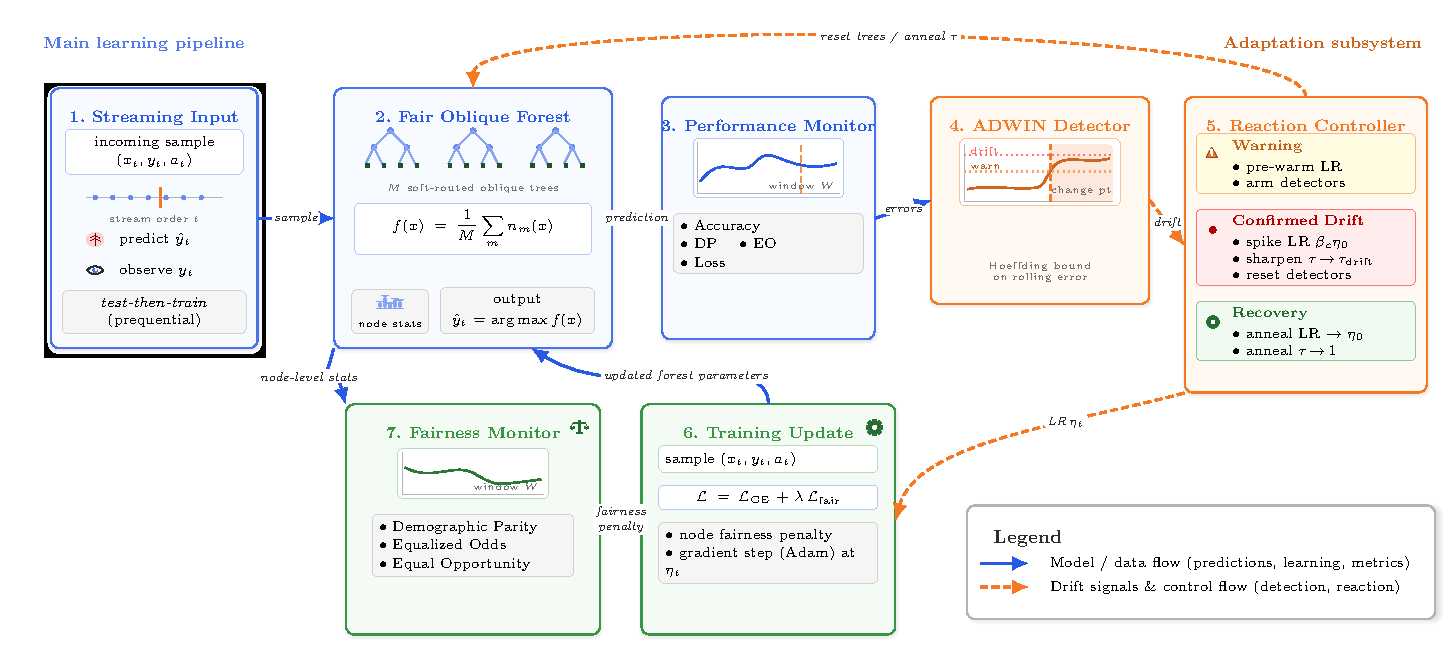
\includegraphics[width=0.85\textwidth]{fado_figure}
\caption{The \textsc{FADO} online learning system. The \emph{main learning pipeline} (blue) streams each sample $(x_t,y_t,a_t)$ through the \textsc{Aranyani} fair oblique
forest~\cite{chowdhury2024enhancing} under a prequential test-then-train protocol, monitors prequential accuracy and the intersectional fairness metrics over a rolling
window of size $W$, and applies the fairness-regularised gradient update $\mathcal{L}=\mathcal{L}_{\mathrm{CE}}+\lambda\mathcal{L}_{\mathrm{fair}}$, which writes the updated
parameters back to the forest. The \emph{adaptation subsystem} (orange) runs the dual-threshold ADWIN detector and the reaction controller, which on a confirmed drift spikes
the learning rate $\eta_t$ and sharpens the soft-routing temperature $\tau_t$, then anneals both back during recovery. Solid blue arrows denote the model/data flow; dashed
orange arrows denote drift signals and control flow.}
\Description{A system diagram of the FADO online learning framework arranged as
seven rounded modules on a light background. A blue-tinted region groups the
main learning pipeline: Streaming Input, Fair Oblique Forest, Performance
Monitor on the top row, and Fairness Monitor and Training Update on the bottom
row. An orange-tinted region groups the adaptation subsystem: the ADWIN drift
detector and the reaction controller, whose Warning, Confirmed-Drift and
Recovery phases are colour coded. Solid blue arrows carry data and model flow
between modules; dashed orange arrows carry drift signals and control flow,
including a feedback arrow from Training Update back to the Fair Oblique
Forest.}
\label{fig:drift-pipeline}
\end{figure*}
Algorithm~\ref{alg:fado} states the resulting prequential loop in full; the subsections that follow detail each component.

\begin{algorithm}[t]
\caption{\textsc{FADO} prequential test-then-train loop}
\label{alg:fado}
\begin{algorithmic}[1]
\Require stream $\{(x_t,y_t,a_t)\}_{t=1}^{T}$; base LR $\eta_0$; multipliers $\beta_w,\beta_c$; temperatures $\tau,\tau_{\mathrm{drift}}$; ADWIN levels $\delta_w,\delta_c$; window $W$; cooldown $C$; guard $\nu$
\State init forest $f$, optimiser at $\eta_0$, temperature $\tau$
\State init detectors $D_w(\delta_w),\,D_c(\delta_c)$; running fairness stats $S$
\State $\textit{warn}\gets\textsc{false}$;\ \ $t_{\text{last}}\gets-C$;\ \ $\textit{recovering}\gets\textsc{false}$
\For{$t = 1$ \textbf{to} $T$}
  \State $\hat{y}_t \gets \arg\max f(x_t)$;\ \ $e_t \gets \mathbf{1}[\hat{y}_t \neq y_t]$ \Comment{test}
  \State update windowed DP (and marginal DP) over last $W$
  \State $\textit{noise} \gets e_t \wedge (\text{conf}(\hat{y}_t) > \nu)$ \Comment{label-noise guard}
  \If{\textbf{not} $\textit{noise}$}\ $D_w.\textrm{update}(e_t)$;\ $D_c.\textrm{update}(e_t)$ \EndIf
  \If{$D_w$ fired \textbf{and not} $\textit{warn}$ \textbf{and} $t-t_{\text{last}}\!\geq\!C$}
     \State $\eta \gets \beta_w\,\eta_0$;\ \ $\textit{warn}\gets\textsc{true}$ \Comment{pre-warm}
  \EndIf
  \If{$D_c$ fired \textbf{and} $t-t_{\text{last}}\!\geq\!C$}
     \State $\eta \gets \beta_c\,\eta_0$;\ \ $\tau \gets \tau_{\mathrm{drift}}$ \Comment{confirm: spike + sharpen}
     \State reset $D_w,D_c$;\ $t_{\text{last}}\gets t$;\ $\textit{warn}\gets\textsc{false}$;\ $\textit{recovering}\gets\textsc{true}$
  \EndIf
  \If{$\textit{recovering}$ \textbf{and} rolling-acc $\geq$ pre-drift baseline}
     \State anneal $\eta\!\to\!\eta_0$ over $\Delta$;\ \ $\tau\!\to\!1$;\ \ $\textit{recovering}\gets\textsc{false}$
  \EndIf
  \State accumulate fairness stats $S$ from $(a_t,y_t)$ \Comment{train}
  \State $g \gets \nabla\!\big(\mathcal{L}_{\mathrm{CE}}(f(x_t),y_t) + \lambda\,\mathcal{L}_{\mathrm{fair}}(S)\big)$
  \State optimiser step on $f$ with $g$ at rate $\eta$
\EndFor
\end{algorithmic}
\end{algorithm}

All experiments were run in Python 3.9 across three machines: a MacBook Pro (Apple M5, $16$\,GB RAM); a desktop with Intel i5-8500 CPU, NVIDIA GTX $1060$ Ti GPU, and $16$\,GB RAM; and a desktop with Intel i9-9900K CPU, NVIDIA RTX $2080$ Ti GPU, and $32$\,GB RAM. Per-seed runs were dispatched across the three machines for wall-clock parallelism; within any given seed, all four models were executed on the same machine to preserve the seed-pinned data ordering required by the paired statistical tests (Section~\ref{sec:method:protocol}). Source code, configuration files, and seed manifests are released for reproducibility (Section~\ref{sec:method:reproducibility}).

\subsection{Fair Oblique Decision Forest}
\label{sec:method:model}
The base model is an ensemble of $K$ soft-routed oblique decision trees of depth $h$ (Table~\ref{tab:hparams}), each with $2^{h}{-}1$ internal routing nodes
$n_j(x) = \sigma\!\big((w_j^{\top} x + b_j)/\tau\big) \in (0,1)$ (trainable $w_j,b_j$; shared temperature $\tau$) and $2^{h}$ leaves storing class logits $\theta_\ell$. Path
probabilities $p_\ell(x)$ follow from the routing decisions via a pre-computed leaf--subtree mask; the per-tree output is $f_k(x) = \sum_\ell p_\ell(x)\,\theta_\ell$, and the
forest aggregates per-tree softmaxes, $f(x) = \tfrac{1}{K}\sum_{k} \mathrm{softmax}(f_k(x))$, with $\hat{y} = \arg\max_c f_c(x)$. The temperature $\tau$ is the controller's
main lever: at $\tau{=}1$ routing is smooth and gradient-friendly (steady state), while $\tau\!\to\!0$ sharpens routing for decisive recovery after a confirmed drift
(Section~\ref{sec:method:drift}).

\subsection{Fairness-Aware Online Updates}
\label{sec:method:updates}
Following the in-processing strategy of the \textsc{Aranyani} base learner~\cite{chowdhury2024enhancing}, \textsc{FADO} enforces fairness at the level of individual routing
nodes rather than only at the output layer. Per-step learning combines the predictive loss with the node-level fairness penalty introduced in Section~III:
\[
\mathcal{L}_t \;=\; \mathcal{L}_{\mathrm{CE}}\bigl(f(x_t), y_t\bigr) \;+\; \lambda \sum_{(k,j)} \frac{1}{|\mathcal{A}|}\sum_{a \in \mathcal{A}} \phi_\delta\!\bigl(F_{kj,a}\bigr),
\]
where $\mathcal{L}_{\mathrm{CE}}$ is the per-step cross-entropy with logits and $\phi_\delta(\cdot)$ is the piecewise quadratic--linear surrogate of Section~III. The
implementation supports both the DP objective $\mathcal{L}$ above and the EO objective $\mathcal{L}_{\mathrm{EO}}$ of Section~\ref{sec:problem:regulariser} as
selectable optimisation targets, and both fairness statistics are computed and monitored online throughout the prequential stream regardless of which one is being
optimised. The study reported here fixes the optimisation target to the demographic-parity regulariser $\mathcal{L}$: every \textsc{FADO} and \textsc{Aranyani} number
in Section~\ref{sec:results} is produced by minimising intersectional DP, and we report accuracy alongside the intersectional and marginal DP violations. The
companion equalised-odds objective $\mathcal{L}_{\mathrm{EO}}$ --- which maintains a separate class-conditional set of running statistics (one per class per node) and
adds a per-class penalty term, roughly doubling the per-step fairness cost --- is the subject of an ongoing EO-objective sweep whose results are deferred
(Section~\ref{sec:conclusion}); we keep its full derivation in Section~\ref{sec:problem:regulariser} because the same controller and pipeline drive it unchanged.
Symbols and concrete values for $\lambda$, $\delta$, and the remaining hyperparameters are listed in Table~\ref{tab:hparams}.
To keep the update memory-efficient, the fairness gradient state is maintained as five running tensors—per-node weight and bias gradient accumulators, a per-class
output accumulator, a subgroup count, and a per-class subgroup count—initialised once at the start of the stream and updated in place via an exponential moving average
on every observed sample. The fairness contribution to the gradient is then assembled in closed form from these running statistics and added to the predictive gradient
before the optimiser step. This design preserves the parameter-isolation property of the original Aranyani formulation~\cite{chowdhury2024enhancing}: each fairness term
depends only on local node parameters, which keeps the per-step cost linear in the number of nodes and removes any need to store past samples.
Predictive and fairness metrics are computed over the rolling window of size $W$ (Table~\ref{tab:hparams}); using the same window for the reported metric and for the
regulariser ensures that the quantity exposed to the reader is exactly the quantity the model is being trained against, with per-step fairness evaluation in $\mathcal{O}(W)$
rather than $\mathcal{O}(t)$.

\subsection{Drift Detection and Reaction Controller}
\label{sec:method:drift}
The controller observes the online error stream $e_t = \mathbf{1}[\hat{y}_t \neq y_t]$ through two independent ADWIN detectors—a pre-warm detector $D_w$ and a
confirmation detector $D_c$—parameterised by significance levels $\delta_w$ and $\delta_c$. The pre-warm detector is paired with a label-noise guard that excludes a
sample from the change signal whenever an incorrect prediction is emitted with post-softmax confidence above $\nu$, preventing single confident-but-wrong samples from
spuriously activating the controller. A minimum of $m_0$ samples per detector is enforced before the first activation to avoid early-stream false positives.

When $D_w$ fires, the optimiser learning rate is multiplied by $\beta_w$ over the $\Delta$-step horizon, pre-warming the parameters for a potential change. When $D_c$
subsequently confirms a drift, three actions are taken atomically: (i) the learning rate is set to $\beta_c \cdot \eta_0$; (ii) the soft-routing temperature of every tree
is set to $\tau_{\mathrm{drift}}$, sharpening routing decisions while the ensemble re-fits; and (iii) both detectors are reset and a cooldown of $C$ samples is enforced
before a new event can fire. Recovery is signalled when the rolling accuracy returns to the pre-drift baseline (estimated over the preceding window of $W$ samples),
after which $\tau$ is annealed back toward its steady-state value at rate $\Delta\tau$ per step and $\eta$ decays linearly to $\eta_0$ over $\Delta$ steps. Concrete values
for $\delta_w$, $\delta_c$, $\beta_w$, $\beta_c$, $\Delta$, $\tau_{\mathrm{drift}}$, $\Delta\tau$, $C$, $\nu$, and $m_0$ are reported in Table~\ref{tab:hparams}.

The two-stage design balances a confirmation-only reaction (too slow under sudden drift) against pre-warming without a gate (amplifies noise); combined with the
label-noise guard, it separates genuine distributional change from confident-but-wrong predictions, the dominant false-positive mode we observed on the held-out tuning
subset (Section~\ref{sec:method:hpo}).

\subsection{Datasets and Preprocessing}
\label{sec:method:data}
Table~\ref{tab:datasets} summarises the two datasets. \textsc{COMPAS} provides a controlled, low-dimensional testbed on which we can inject synthetic
concept-drift perturbations of a known form on the test stream; \textsc{Folktables} (ACS Income, CA) supplies a large natural cross-year shift between
$2015$ (training) and $2017$--$2018$ (prequential test). Both datasets are processed through a shared tabular pipeline: numerical features are standardised
using training-set means and standard deviations, categorical variables are one-hot encoded, and (for \textsc{COMPAS}) the long-tail \texttt{c\_charge\_desc}
column is frequency-encoded with rare categories collapsed below a count threshold. The encoder is fitted on the training split alone and reused unchanged
for the test stream, so the streaming protocol remains free of test-time information leakage.

\begin{table}[t]
\centering
\caption{Datasets.}
\label{tab:datasets}
\setlength{\tabcolsep}{1pt}
\resizebox{\columnwidth}{!}{%
\begin{tabular}{l p{1.6cm} p{2.2cm} p{2.6cm} p{3.0cm}}
\toprule
Dataset & Size & Target & Protected attribute & Split / stream \\
\midrule
COMPAS & 7{,}214 & Two-year recidivism & Race $\times$ Sex (4 joint groups) & 70/30 stratified train/test (5{,}049/2{,}165); two injected concept-drift scenarios on test stream \\
Folktables (ACS Income, CA) & 187{,}474 + 187{,}475 & Income $> \$50$K & Sex $\times$ Race (4 joint groups) & Train 2015; test 2017--2018; both splits uniformly subsampled to 10\% per seed \\
\bottomrule
\end{tabular}}
\end{table}

\subsection{Concept-Drift Scenarios}
\label{sec:method:scenarios}
We adopt complementary strategies on the two streamed datasets. On \textsc{COMPAS} the original distribution is approximately stationary, so we
inject a synthetic, parametrically controlled concept-drift perturbation on the test stream: this isolates the abrupt label-correlated subpopulation-shift
regime that the dual-ADWIN controller is designed to detect, and lets us read its effect off the prequential curves under a known ground truth. On \textsc{Folktables} (ACS Income, CA), training on $2015$ and evaluating prequentially on $2017$--$2018$ already provides a real,
multidimensional cross-year shift driven by genuine demographic and economic change; injecting additional synthetic perturbations on top of it would
conflate the controlled and natural signals and obscure the source of any observed degradation. We therefore use \textsc{Folktables} as an
unmanipulated natural-drift testbed and reserve the controlled scenarios below for \textsc{COMPAS}.

Each scenario combines (i) a row-level edit of the \texttt{race} categorical feature in the test stream with (ii) a stochastic flip of the
\texttt{two\_year\_recid} label on the same edited rows. The label flip is sampled independently per edited row as $\mathrm{Bernoulli}(0.5)$, so the
flipped subset is a random half of the affected subpopulation rather than every row. The choice of $p=0.5$ is a design decision of the testbed
\emph{a priori}, not a value tuned against the test-stream metrics: at $p=1.0$ the flip is deterministic and the model can simply learn the inverted
rule, making the drifted regime trivially separable in the opposite direction; at $p=0.0$ no label change occurs and the perturbation reduces to virtual
covariate drift. Bernoulli($0.5$) is the maximally entropic midpoint at which the post-drift labelling is unlearnable for the affected subpopulation,
ensuring the scenario tests recovery rather than re-learning. Pairing the categorical edit with the per-subgroup label flip moves $P(y \mid x)$ as well
as $P(x)$ for the affected subpopulation, yielding genuine concept drift~\cite{DBLP:journals/corr/WebbHCNP15} rather than purely virtual covariate drift.

The test stream is partitioned into \emph{Warmup} ($0$--$30\%$, $\sim 650$ samples), \emph{Drift} ($30$--$70\%$, $\sim 865$), and \emph{Recovery}
($70$--$100\%$, $\sim 650$); the edit-and-flip is applied only during the drift phase. The two active scenarios are: \emph{no\_drift}, the original
distribution preserved throughout (any drift event fired here is a false positive of the detector); and \emph{abrupt\_race}, a symmetric AA$\leftrightarrow$Caucasian swap sustained
across the drift phase with a $\mathrm{Bernoulli}(0.5)$ \texttt{two\_year\_recid} flip on the same rows.
\subsection{Baselines}
\label{sec:method:baselines}
We compare \textsc{FADO} against three streaming baselines that span the accuracy/fairness/adaptivity design space:
\begin{itemize}
  \item \textbf{ARF}~\cite{10.1007/s10994-017-5642-8}: the Adaptive Random Forest from the \texttt{river} library, used as an accuracy-oriented streaming reference that handles drift through per-tree warning and drift detectors and background trees, but without any fairness mechanism;
  \item \textbf{RFR}: a sharpness-aware reweighting variant that applies the RFR optimiser~\cite{jiang2023chasingfairnessdistributionshift} (sharpness-aware minimisation over a fairness-reweighted loss); this provides a fairness-aware static baseline without adaptive drift handling;
  \item \textbf{Aranyani}~\cite{chowdhury2024enhancing}: the bare \textsc{Aranyani} forest with the node-level fairness regulariser active but the dual-ADWIN detector and reaction controller disabled. This is the strict controller-ablation of \textsc{FADO} --- same base learner, same loss, same rolling-window stats, same seed-pinned data ordering --- so any \textsc{FADO}-vs-\textsc{Aranyani} gap is attributable to the controller alone.
\end{itemize}
All baselines are evaluated under the same batch-size-one test-then-train prequential protocol as \textsc{FADO} so that comparisons are not confounded by data ordering or by access to look-ahead information. The global RNG (NumPy, Python \texttt{random}, and TensorFlow) is pinned per seed before each model is instantiated, so the data split, the forest initialisation, and the training trajectory are bit-identical across methods that share a seed---paired statistical tests therefore compare points that differ \emph{only} in the method under evaluation.

\subsection{Hyperparameter Selection}
\label{sec:method:hpo}
Table~\ref{tab:hparams} lists the fairness-regulariser and controller hyperparameters with their Folktables defaults and the COMPAS overrides. For the base learner we use $K=4$ trees of depth $h=4$ with base learning rate $\eta_0=2{\times}10^{-3}$, slightly larger than the \textsc{Aranyani} defaults to handle Folktables' higher dimensionality. The non-obvious overrides are justified below.

\begin{table}[t]
\centering
\caption{\textsc{FADO} hyperparameters. Dash = \textsc{COMPAS} inherits the \textsc{Folktables} default.}
\label{tab:hparams}
\setlength{\tabcolsep}{3pt}
\resizebox{\columnwidth}{!}{%
\begin{tabular}{l c c p{3.4cm}}
\toprule
\textbf{Symbol} & \textbf{Folktables} & \textbf{COMPAS} & \textbf{Role} \\
\midrule
\multicolumn{4}{l}{\emph{Fairness regulariser}} \\
\midrule
$\lambda$   & $1.0$               & --                  & Fairness-penalty weight \\
$\delta$    & $0.1$               & --                  & Quadratic/linear transition point in $\phi_\delta$ \\
$\gamma$    & $0.9$               & --                  & EMA decay of running fairness statistics \\
$W$         & $1000$              & $250$               & Rolling window for $\mathbb{E}[\cdot]$ and reported DP \\
\midrule
\multicolumn{4}{l}{\emph{Drift controller}} \\
\midrule
$\delta_w$  & $1 \times 10^{-5}$  & $1 \times 10^{-3}$  & ADWIN significance (pre-warm detector) \\
$\delta_c$  & $2 \times 10^{-2}$  & $2 \times 10^{-1}$  & ADWIN significance (confirmation detector) \\
$\beta_w$   & $5$                 & --                  & LR multiplier on warning \\
$\beta_c$   & $10$                & --                  & LR multiplier on confirmed drift \\
$\Delta$    & $3000$              & $600$               & LR decay horizon back to $\eta_0$ \\
$\tau$              & $1.0$       & --                  & Steady-state soft-routing temperature \\
$\tau_{\mathrm{drift}}$ & $0.1$   & --                  & Temperature set on confirmed drift \\
$\Delta\tau$ & $2 \times 10^{-3}$ & --                  & Per-step temperature anneal back to $\tau$ \\
$C$         & $200$               & --                  & Cooldown (samples) between consecutive events \\
$\nu$       & $0.7$               & --                  & Label-noise confidence guard \\
$m_0$       & $30$                & $20$                & Min.\ samples per detector before first activation \\
\bottomrule
\end{tabular}}
\end{table}

The per-dataset overrides follow from a single closed-form scaling argument: ADWIN's cut threshold scales as $\varepsilon_{\mathrm{cut}} = \sqrt{(1/2m)\ln(4/\delta)}$, so
shorter streams need a looser $\delta$ and a proportionally shorter window $W$, LR horizon $\Delta$, and activation count $m_0$ to react within a single drift phase --- which
is why the $\sim$$2$k-sample \textsc{COMPAS} stream loosens $\delta_c$ by two orders of magnitude and drops $W$ to $250$ relative to \textsc{Folktables}. The fairness weight
$\lambda$ is selected per dataset on a held-out portion of the training split alone --- the test stream is never consulted --- via a compact NSGA-II search on
\textsc{Folktables} and a one-dimensional grid on \textsc{COMPAS}; both converge to $\lambda=1$. The remaining per-step knobs are stream-length-independent and held fixed
across datasets. Appendix~\ref{app:hpo} gives the full per-knob derivation, including the label-noise guard $\nu=0.7$ that suppresses the dominant false-positive mode.

\subsection{Evaluation Protocol}
\label{sec:method:protocol}
All methods are evaluated under a strict prequential, batch-size-one, test-then-train protocol: at each step the model emits $\hat{y}_t$, the prequential metrics
are updated, and only then is the parameter update performed using the just-observed $(y_t, a_t)$. We report mean and standard deviation over $30$ seeds.
The primary metrics are prequential accuracy and the \emph{intersectional} demographic-parity violation (DP) over the four joint sex\,$\times$\,race subgroups,
computed over the same $W$-sample rolling window that drives the fairness regulariser (Table~\ref{tab:hparams}). As transparency diagnostics we additionally report
the two \emph{marginal} per-attribute DP violations ($\mathrm{DP}_{\text{sex}}$, $\mathrm{DP}_{\text{race}}$), each obtained by projecting the joint subgroup index onto
a single attribute and applying the same DP definition over the full prediction stream. For \textsc{COMPAS}, each (seed, model) cell produces one prequential value per
scenario over the full test stream; the two scenarios are then averaged within each seed before aggregation. For \textsc{Folktables}, each (seed, model) cell produces
one prequential value over the per-seed $10\%$ subsample of the $2017$--$2018$ test stream. In both cases the table reports mean $\pm$ standard deviation across the $30$
seeds.

For each metric column, paired-by-seed comparisons of \textsc{FADO} against each baseline are performed using the two-sided Wilcoxon signed-rank test;
$p$-values are corrected within each column using the Holm--Bonferroni step-down procedure across the three baselines. The procedure follows the
prequential-benchmark recommendations of Dem{\v{s}}ar~\cite{demsar2006statistical}; the rationale for choosing paired Wilcoxon over the Welch
two-sample $t$-test is discussed in Appendix~\ref{app:tests}.

\subsection{Reproducibility}
\label{sec:method:reproducibility}
The full implementation, configuration files, seed manifests, and per-seed result files are released at
\url{https://github.com/TiagoSilva35/Aranyani2.0}. The repository's \texttt{README.md} reproduces Table~\ref{tab:results} and lists, for each dataset, the
exact command-line invocation that produced every reported row (per-seed sweep, paired Wilcoxon + Welch significance run, summary aggregation). Running the
commands as listed regenerates the same per-seed \texttt{results.json} files that the reported means, standard deviations, and Holm-corrected $p$-values
are computed from.

\section{Results and Discussion}
\label{sec:results}
We report the intersectional (sex\,$\times$\,race) setting on the natural cross-year shift of \textsc{Folktables} (Table~\ref{tab:results}), as mean $\pm$ std
over $30$ seeds, with the demographic-parity regulariser as the optimisation target. The table gives accuracy, the intersectional DP that \textsc{FADO}
optimises, and the two marginal per-attribute DP diagnostics. The controlled abrupt-shift \textsc{COMPAS} testbed under intersectional grouping, and the
equalised-odds objective, are pending the companion sweep (Section~\ref{sec:conclusion}); the \textsc{COMPAS} rows of Table~\ref{tab:results} are marked
accordingly.

\begin{table}[!htbp]
\centering
\caption{Prequential results under \emph{intersectional} (sex\,$\times$\,race) grouping, mean $\pm$ std over $30$ seeds. DP is the intersectional demographic-parity violation over the four joint subgroups (the objective \textsc{FADO} optimises); $\mathrm{DP}_{\text{sex}}$ and $\mathrm{DP}_{\text{race}}$ are the marginal per-attribute diagnostics. \textbf{Bold} = best mean per metric within each dataset; superscripts on the \textsc{FADO} row = paired Wilcoxon Holm-corrected significance vs \emph{every} baseline ($^{*}p{<}0.05$, $^{**}p{<}0.01$, $^{***}p{<}0.001$); columns with no marker have mixed per-baseline directions and are dissected in the text. Equalised-odds results are deferred to the EO-objective study (Section~\ref{sec:conclusion}).}
\label{tab:results}
\setlength{\tabcolsep}{3pt}
\resizebox{\columnwidth}{!}{%
\begin{tabular}{llcccc}
\toprule
Dataset & Model & Accuracy $\uparrow$ & DP $\downarrow$ & $\mathrm{DP}_{\text{sex}}\!\downarrow$ & $\mathrm{DP}_{\text{race}}\!\downarrow$ \\
\midrule
\multirow{4}{*}{\textsc{Folktables}}
 & \textbf{FADO} & $0.7979 \pm 0.0066$ & $\mathbf{0.0688 \pm 0.0057}^{***}$ & $\mathbf{0.0234 \pm 0.0064}^{***}$ & $\mathbf{0.0243 \pm 0.0051}^{***}$ \\
 & Aranyani      & $\mathbf{0.8005 \pm 0.0054}$ & $0.0727 \pm 0.0050$ & $0.0283 \pm 0.0036$ & $0.0294 \pm 0.0035$ \\
 & ARF           & $0.7446 \pm 0.0107$ & $0.1497 \pm 0.0144$ & $0.0735 \pm 0.0126$ & $0.0620 \pm 0.0070$ \\
 & RFR           & $0.7779 \pm 0.0044$ & $0.1427 \pm 0.0073$ & $0.0724 \pm 0.0059$ & $0.0591 \pm 0.0048$ \\
\midrule
\multirow{4}{*}{\textsc{COMPAS}}
 & \textbf{FADO} & \TODO{} & \TODO{} & \TODO{} & \TODO{} \\
 & Aranyani      & \TODO{} & \TODO{} & \TODO{} & \TODO{} \\
 & ARF           & \TODO{} & \TODO{} & \TODO{} & \TODO{} \\
 & RFR           & \TODO{} & \TODO{} & \TODO{} & \TODO{} \\
\bottomrule
\end{tabular}}
\end{table}

\subsection{RQ1: To What Extent Does Concept Drift Affect Group Fairness?}
\label{sec:results:rq1}
The \textsc{Folktables} cross-year shift inflates the intersectional fairness violation of both external streaming baselines (Table~\ref{tab:results}).
\textsc{ARF}, which carries no fairness mechanism, lands at intersectional $\mathrm{DP}=0.1497$ on the $2017$--$2018$ stream against \textsc{FADO}'s $0.0688$.
\textsc{RFR}, which \emph{is} fairness-aware via sharpness-aware reweighting fitted on the $2015$ training data, nonetheless drifts to $\mathrm{DP}=0.1427$ on the
same test stream --- more than double \textsc{FADO}'s --- despite enforcing fairness at training time, which directly illustrates the static-fairness failure mode
(L1 in Section~\ref{sec:related:limitations}). Both gaps are highly significant (paired Wilcoxon Holm-corrected $p<0.001$). Crucially, the controller-free
\textsc{Aranyani} baseline lands close to \textsc{FADO} ($\mathrm{DP}=0.0727$), so the bulk of the gap to \textsc{ARF} and \textsc{RFR} is contributed by the
\emph{in-processing} fairness regulariser, not by the controller.

A finding unique to the intersectional view is that the disparity drift leaves behind is \emph{concentrated in the joint subgroups}. Measuring each method's
intersectional DP against its worst marginal DP, the unconstrained and statically-fair baselines sit at a ratio of $\approx\!2.0$ (\textsc{ARF} $0.1497/0.0735$,
\textsc{RFR} $0.1427/0.0724$), whereas the in-processing fair learners are \emph{higher} still --- \textsc{FADO} $0.0688/0.0243\approx2.8$, \textsc{Aranyani}
$0.0727/0.0294\approx2.5$ --- because they scrub the marginal axes so effectively that their residual unfairness is proportionally more intersectional. A
marginal-only audit would therefore have declared \textsc{FADO} ``very fair'' ($\mathrm{DP}_{\text{sex}}{=}0.0234$, $\mathrm{DP}_{\text{race}}{=}0.0243$) while
missing a joint-subgroup gap roughly $2.8\times$ larger: the fairness-gerrymandering construction of~\cite{kearns2018gerrymandering} manifesting on real data, and
the empirical justification for optimising the intersectional objective directly rather than the per-axis marginals.

\subsection{RQ2: Can Adaptive Mechanisms Preserve Fairness While Maintaining Utility?}
\label{sec:results:rq2}
\textsc{FADO} attains the best mean intersectional DP and the best marginal DP on both axes against both external streaming baselines (\textsc{ARF} and
\textsc{RFR}), and beats them on accuracy as well (Table~\ref{tab:results}). On \textsc{Folktables} this manifests as $+5.3$pp accuracy over \textsc{ARF} and
$+2.0$pp over \textsc{RFR}, a $\sim 54\%$/$\sim 52\%$ intersectional-DP reduction, and a corresponding reduction on both marginal axes; all twelve
FADO-vs-\{\textsc{ARF},\textsc{RFR}\} comparisons across the four reported metrics reach Holm-corrected paired Wilcoxon $p<0.001$, and every one of them is also
significant under the more conservative Welch $t$-test. The RQ2 answer against the accuracy-only and the fairness-without-adaptation baselines is therefore
unambiguous: an adaptive in-processing fairness-aware learner produces the highest mean on accuracy and the lowest mean on every DP statistic, intersectional
and marginal, with every win highly significant under both tests.

The \textsc{FADO}-vs-\textsc{Aranyani} comparison isolates the contribution of the reaction controller itself: the two models share the identical base
learner, fairness loss, rolling-window statistics, and seed-pinned data ordering, so the gap between the two rows is attributable solely to the dual-ADWIN
controller. The intersectional setting surfaces a controller benefit that the single-attribute view did not: the controller reduces intersectional DP by
$0.38$pp in \textsc{FADO}'s favour, and --- unlike the sub-$0.3$pp differences typical of this gradual-shift comparison --- this reduction is significant under
\emph{both} the paired Wilcoxon ($p<0.001$) \emph{and} the Welch $t$-test ($p<0.01$), as is the corresponding $0.49$pp/$0.51$pp reduction on the marginal sex
and race axes (both $p<0.001$ under both tests). The single cost is a $0.26$pp accuracy deficit in \textsc{Aranyani}'s favour, which is flagged by the
sign-consistency Wilcoxon ($p<0.001$) but is \emph{not} distinguishable under Welch ($p=0.10$) because it sits well inside the seed-to-seed spread
(Appendix~\ref{app:tests}). The interpretation is that the larger joint-subgroup target gives the spike-then-anneal controller more fairness signal to
act on than any single marginal axis does: optimising over four cells rather than two amplifies the per-step fairness gradient the controller modulates, so the
controller's contribution becomes measurable even on the smooth cross-year shift where the single-attribute controller was statistically tied. RQ2 is therefore
answered affirmatively: \textsc{FADO} wins decisively against the accuracy-only and static-fair baselines, and the reaction controller adds a both-tests-significant
intersectional-DP improvement over the controller-free base learner at a Welch-negligible accuracy cost.

\section{Conclusion and Future Work}
\label{sec:conclusion}
We introduced \textsc{FADO}, which wraps the \textsc{Aranyani} fair oblique decision forest (the inherited in-processing base learner) with an ADWIN-driven
dual-threshold detector and a reaction controller that spikes the learning rate and sharpens the soft-routing temperature on confirmed drift and anneals both back
during recovery; the contribution is the drift-detection-and-response machinery and its intersectional fairness instantiation.

Empirically, on \textsc{Folktables} under intersectional (sex\,$\times$\,race) grouping over $30$ seeds, optimising demographic parity, \textsc{FADO} more than halves
the intersectional DP of \textsc{ARF} and \textsc{RFR} (all twelve comparisons at Holm-corrected $p<0.001$ under both tests) and, unlike the single-attribute setting,
beats the controller-free \textsc{Aranyani} base learner by a both-tests-significant margin (Wilcoxon $p<0.001$, Welch $p<0.01$) at a Welch-negligible $0.26$pp accuracy
cost --- the larger four-cell objective gives the controller more fairness signal to act on (RQ2). Residual disparity, for \emph{every} method including the fair
learners, stays concentrated in the joint subgroups (intersectional-to-marginal ratio $\approx\!2$--$3$), reproducing the fairness-gerrymandering
construction~\cite{kearns2018gerrymandering} on real data and justifying intersectional over marginal optimisation (RQ1).

The most immediate extension is the \emph{equalised-odds objective}: the EO regulariser (Appendix~\ref{app:eo}) is driven by the same controller, and a companion sweep
optimising EO directly --- with the intersectional \textsc{COMPAS} testbed left as placeholders in Table~\ref{tab:results} --- is underway. Further directions include
time-resolved fairness metrics, extension to $K>2$ groups, and a component ablation of the controller's branches.

\newpage
\bibliographystyle{ACM-Reference-Format}
\bibliography{references}

\appendix

\section{Equalised Odds: Metric and Regulariser}
\label{app:eo}
\emph{Equalised odds} (EO) is the label-conditional fairness notion that compares group prediction rates separately within each true-label class. For each $y \in \{0,1\}$,
$\hat{p}_{a|y} = \mathbb{E}[\hat{y} \mid a, y]$ is the positive-prediction rate of group $a$ within class $y$ and $\bar{p}_y = \frac{1}{|\mathcal{A}_t|}\sum_{a'}\hat{p}_{a'|y}$ its
cross-group mean; the EO violation is the worst-case deviation across both classes,
\[
\mathrm{EO} = \max_{y \in \{0,1\}} \max_{a \in \mathcal{A}_t}\left|\hat{p}_{a|y} - \bar{p}_y\right|,
\]
and restricting the outer maximisation to $y{=}1$ yields equal opportunity. EO disentangles bias from class imbalance and is informative when base rates differ across groups.

The companion equalised-odds objective referenced in Section~\ref{sec:method:updates} conditions each running statistic on the true label. For $c \in \{0,1\}$:
\[
\bar{n}_{ij,a|c} = \mathbb{E}[n_{ij}(x) \mid y=c, a], \qquad
\bar{n}_{ij|c} = \frac{1}{|\mathcal{A}|}\sum_{a' \in \mathcal{A}} \bar{n}_{ij,a'|c},
\]
where $\bar{n}_{ij,a|c}$ is the group-and-label-conditional average routing decision at node $(i,j)$ (the per-node analogue of $\hat{p}_{a|y}$) and $\bar{n}_{ij|c}$ is its
cross-group mean within class $c$. The corresponding node deviation and EO regulariser are:
\[
F_{ij,a}^{(c)} = \bar{n}_{ij|c} - \bar{n}_{ij,a|c},
\]
\[
\mathcal{L}_{\text{EO}} = \lambda \sum_{(i,j)} \frac{1}{2|\mathcal{A}|}\sum_{c \in \{0,1\}}\sum_{a \in \mathcal{A}} \phi_{\delta}\!\left(F_{ij,a}^{(c)}\right),
\]
which differs from the DP regulariser only by the additional sum over $c$ and the corresponding $\tfrac{1}{2}$ normalisation; the rest of the structure (per-node penalty,
group average, $\phi_\delta$ surrogate) is identical. The same dual-ADWIN controller and prequential loop (Algorithm~\ref{alg:fado}) drive it without modification.

\section{Per-Dataset Hyperparameter Calibration}
\label{app:hpo}
This appendix expands the per-dataset overrides summarised in Table~\ref{tab:hparams} and referenced in Section~\ref{sec:method:hpo}.
All per-dataset overrides follow from one closed-form scaling argument and one pilot-calibration observation. ADWIN's cut threshold scales as
$\varepsilon_{\mathrm{cut}} = \sqrt{(1/2m)\ln(4/\delta)}$, so for fixed $\delta$ the minimum detectable accuracy deficit grows as $1/\sqrt{m}$: shorter
streams need a looser $\delta$ to detect drifts of equivalent magnitude. On \textsc{Folktables} the long stream tolerates a tight bound ($\delta_w{=}10^{-5}$,
$\delta_c{=}2{\times}10^{-2}$, sub-1\,pp floor); on \textsc{COMPAS} the same $\delta_c$ yields an $\sim$$9$\,pp floor that exceeds the actual deficits during the
$\sim$$865$-sample drift phase, so we loosen by two orders of magnitude ($\delta_w{=}10^{-3}$, $\delta_c{=}2{\times}10^{-1}$). The LR decay horizon $\Delta$
and the minimum activation count $m_0$ are scaled proportionally to stream length so the controller can complete a full spike/decay cycle and so it
does not fire on early-stream noise. The rolling window $W$ is set so it turns over within a single drift phase: $W=1000$ covers $0.27\%$ of the
\textsc{Folktables} stream but would cover $46\%$ of the \textsc{COMPAS} stream, so we drop $W$ to $250$ on \textsc{COMPAS}, matched to ADWIN's
$\sim$$200$-sample bucket scale.
The fairness weight $\lambda$ is the only knob with a non-geometric calibration and is selected per dataset on a held-out portion of the training split
alone --- the test stream is never consulted. On \textsc{Folktables}, a compact NSGA-II procedure (population $8$, $4$ generations) jointly minimises
prequential $1{-}\mathrm{Accuracy}$ and DP on the held-out training subset and picks from the first Pareto front the candidate that minimises the
normalised sum of objectives; this yields $\lambda=1$. On \textsc{COMPAS} the held-out training subset is too small to support a multi-generation NSGA-II
reliably, so we run the same prequential-on-training procedure over a one-dimensional grid $\lambda \in \{0.1, 1, 10\}$ and select the value that
minimises the same combined objective on the held-out training subset; this also yields $\lambda=1$. The two datasets therefore converge on the same
value: at $\lambda=10$ the per-step fairness gradient dominates the classification gradient and the in-sample DP/accuracy product on the held-out subset
degrades; at $\lambda=0.1$ the regulariser contribution becomes too small for the in-sample DP estimate to track group statistics responsively.
The remaining knobs are stream-length-independent per-step quantities and are held fixed across both datasets at the Table~\ref{tab:hparams} values.
The surrogate transition $\delta=0.1$ is inherited from \textsc{Aranyani} and gives a quadratic regime for routing deviations below $10$pp and a
linear regime above, so single-sample gradient noise is treated smoothly while outlier deviations are kept bounded. The EMA decay $\gamma=0.9$
corresponds to an effective half-life of $\sim 7$ samples, fast enough to track per-phase distributional change but slow enough to suppress
single-sample noise. The asymmetric LR multipliers $\beta_w{=}5$ and $\beta_c{=}10$ enforce a $2{:}1$ confirmation/warning ratio: warnings produce
a measurable pre-warm without committing the model to a regime change, and only confirmation triggers the full spike. The drift-time temperature
$\tau_{\mathrm{drift}}=0.1$ (a tenfold reduction from steady-state $\tau=1.0$) makes routing essentially hard for the duration of the spike, so the
ensemble can commit to a different leaf assignment within a few dozen samples rather than waiting for soft-routing weights to average over the
inverted regime; the per-step anneal $\Delta\tau=2{\times}10^{-3}$ returns $\tau$ from $0.1$ to $1.0$ over $450$ steps, which fits inside the
$\Delta=600$ LR decay horizon on \textsc{COMPAS} and synchronises temperature recovery with the LR schedule. The cooldown $C=200$ prevents
re-firing during the controller's own response and is matched to ADWIN's $\sim 200$-sample bucket scale. The label-noise confidence guard $\nu=0.7$
excludes high-confidence-but-wrong predictions from the pre-warm error stream: on the same held-out training subset used for $\lambda$ calibration,
single samples where the forest emitted a high-confidence prediction that disagreed with the noisy ground truth were the dominant false-positive mode,
and a $0.7$ threshold removed them without measurably affecting in-sample true-positive detection of distributional change.

\section{Choice of Statistical Test}
\label{app:tests}
We report the paired Wilcoxon signed-rank test as the primary statistic, following the prequential-benchmark recommendations of
Dem\v{s}ar~\cite{demsar2006statistical}: it makes no parametric assumption about the per-seed metric distribution, and it exploits the within-seed pairing
produced by the shared data ordering (Section~\ref{sec:method:baselines}), which is precisely the structure that makes the Welch two-sample $t$-test
discard relevant information. In the intersectional setting the two tests \emph{agree} on every DP comparison in Table~\ref{tab:results} --- including the
\textsc{FADO}-vs-\textsc{Aranyani} controller-isolation gap, which clears Welch at $p<0.01$ (intersectional) and $p<0.001$ (both marginals) --- so the
fairness conclusions do not hinge on the choice of test. The two tests disagree on exactly one cell: the $0.26$pp \textsc{FADO}-vs-\textsc{Aranyani} accuracy
deficit, which is small in magnitude but consistent in sign. There Welch is non-significant ($p=0.10$, the gap is within the standard deviation of either model
in isolation) while paired Wilcoxon flags it because the sign of the per-seed difference is consistent across $25$+ of the paired seeds. Both numbers are
correct; they answer different questions. Welch asks whether the two models' marginal distributions differ; paired Wilcoxon asks whether the controller
systematically shifts the per-seed outcome in one direction. We report both, and note that the accuracy cost of the controller is negligible under the
distributional reading and merely systematic-but-tiny under the paired reading.

\end{document}
